\documentclass{beamer}
\usetheme{Madrid}
\newcommand{\vect}[1]{\mathbf{#1}}
\title{Rivers and Bridges}
\author{A. Writer}
\begin{document}
\begin{frame}
  \titlepage
\end{frame}
\section{Crossings}
\begin{frame}{Three crossings}
  \begin{itemize}
    \item<1-> The north bridge carries $\vect{v}_1$ trains.
    \item<2-> The ferry runs every \alert{forty} minutes.
    \item<3-> A tunnel is planned for 2031.
  \end{itemize}
  \note{Mention the ferry timetable.}
\end{frame}
\begin{frame}{A sketch}
  \begin{columns}
    \column{0.45\textwidth}
    Left bank, with a pier.
    \column{0.5\textwidth}
    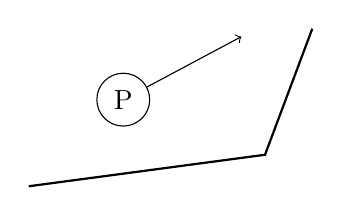
\begin{tikzpicture}
      \draw[thick] (0,0) -- (3,0.4) -- (3.6,2);
      \node[draw,circle] (p) at (1.2,1.1) {P};
      \draw[->] (p) -- (2.7,1.9);
    \end{tikzpicture}
  \end{columns}
\end{frame}
\section{Costs}
\begin{frame}{Estimate}
  \begin{block}{Total}
    Steel: 41 units. \pause Labour: 17 units.
  \end{block}
  \only<2>{Overruns are likely.}
  \[ c = \sum_{i=1}^{3} w_i \]
\end{frame}
\end{document}
